\documentclass[../main.tex]{subfiles}

\begin{document}

\chapter{ Fundemental Group }

\section{Basic Constructions}
\begin{definition}{Product path}{}
Let $X$ be a topological space. Let $\omega, \tau: \mathbb{I} \longrightarrow X$ be two paths such that the terminal point $\omega(1)$ of $\omega$ is the same as the initial point $\tau(0)$ of $\tau$. We then define $\omega * \tau: \mathbb{I} \longrightarrow X$ by the formula
\begin{equation}
\omega * \tau(t)=\left\{\begin{array}{ll}
\omega(2 t), & 0 \leq t \leq 1 / 2, \\
\tau(2 t-1), & 1 / 2 \leq t \leq 1 .
\end{array}\right.
\end{equation}
\end{definition}
\begin{lemma}{}{}
If $\omega_{1} \simeq \omega_{2}$ and $\tau_{1} \simeq \tau_{2}$ and $\omega_{1} * \tau_{1}$ is defined then $\omega_{2} * \tau_{2}$ is defined and we have, $\omega_{1} * \tau_{1} \simeq \omega_{2} * \tau_{2}$.
\end{lemma}

\begin{definition}{}{}
    We can use the standard parameterisation of any closed interval $[a, b]$ by the interval $[0, 1]$ and think of a map $\gamma : [a, b] \to X$ as a path in $X$, viz.,
\[
\hat{\gamma}(t) := \gamma((b - a)t + a).
\]
\end{definition}

\begin{theorem}{Invariance under subdivision}{}
Let $\gamma : [0,1] \to X$ be a path, and $0 < t_1 < \dots < t_n < 1$. Then $\gamma$ is path homotopic to $\widehat{\gamma|_{[0,t_1]}} * \dots * \widehat{\gamma|_{[t_n,1]}}$.
\end{theorem}

\begin{definition}{inverse path}{}
    For a path \(  f  \) from \(  x_0  \)to \(  x_1  \), the \dfntxt{inver path} \(  \bar{f}  \) from \(  x_1  \) back to \(  x_0  \) is defined by \[
    \bar{f}\left( s \right)= f\left( 1-s \right)  
    \]      
\end{definition}

\begin{proposition}{}{}
    Let \(  f  \) is a path from \(  x_0  \) to \(  x_1  \), \(  \bar{f}  \) is the  inverse path.    Then \(  f* \bar{f}  \) and \(  \bar{f}*f  \) are null homotopy.  
\end{proposition}

\begin{proofsketch}
    定义截断路径 \(  f_{t}\left( s \right)   \), 先沿着路径走 \(  \left( 1-t \right)   \)时间 , 走到 \(  f\left( 1-t \right)   \),  再在 \( f\left( 1-t \right)  \)处停留 \(  t  \)时间.    
\end{proofsketch}

\begin{proof}
     Define \[
     f_{t}\left( s \right)= \begin{cases} f\left( s \right),& 0\le s\le 1-t\\ 
      f\left( 1-t \right),& 1-t\le s\le 1   \end{cases}  
     \] Let \(  g_{t} = \overline{f_{t}}  \) , we have \[
     g_{t}\left( s \right)= f_{t}\left( 1-s \right)= \begin{cases} f\left( 1-t\right),& 0\le  s\le t \\ 
      f\left( 1-s \right),& t\le s\le 1  \end{cases}   
     \]  Define \(  h_{t}= f_{t}*g_{t}  \), then define \(  H: I\times I\to X  \),  \(  H\left( s,t \right)= h_{t}\left( s \right)    \).    \[
   \begin{aligned}
     H\left( s,t \right)= h_{t}\left( s \right)&= \begin{cases} f_{t}\left( 2s \right),& 0\le s\le \frac{1}{2}\\ 
      g_{t}\left( 2s-1 \right),& \frac{1}{2}\le s\le 1   \end{cases}  \\ 
       &= \begin{cases} f\left( 2s \right),& 0\le 2s\le 1-t \\ 
        f\left( 1-t \right),& 1-t\le 2s\le 1 \\ 
         f\left( 1-t \right),& 0\le 2s-1\le t\\ 
          f\left( 2-2s\right),& t\le 2s-1\le 1   \end{cases} \\ 
           &= \begin{cases} f\left( 2s \right),&0\le s\le \frac{1-t }{2 }\\ 
            f\left( 1-t \right),& \frac{1-t }{2 }\le s\le \frac{t+ 1 }{2 }\\ 
             f\left( 2-2s \right),&\frac{t+ 1 }{2 }\le s\le 1        \end{cases} 
   \end{aligned}  
     \]

    \begin{center}
       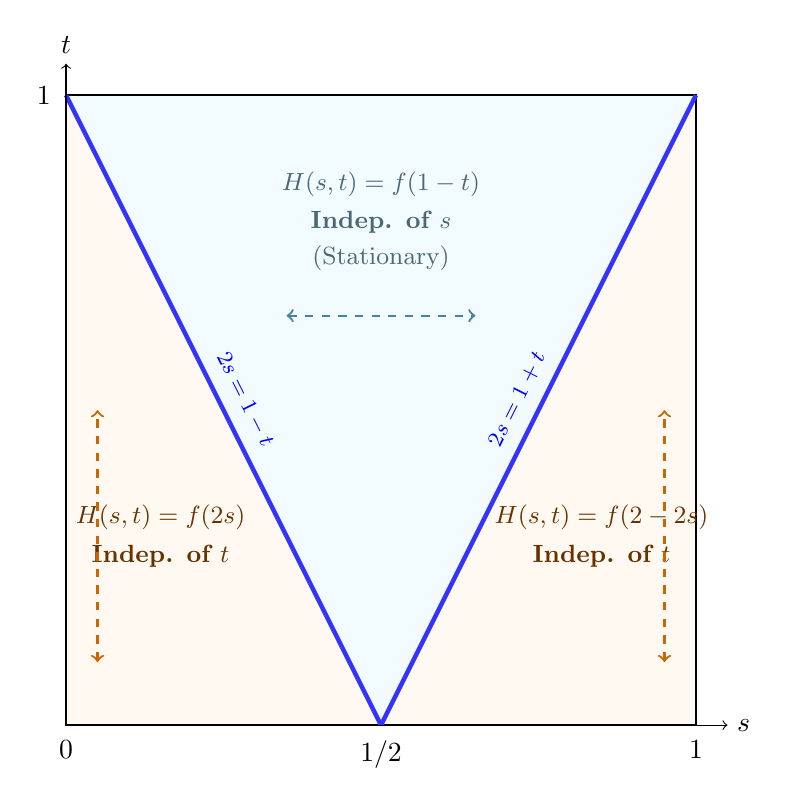
\begin{tikzpicture}[scale=8] % 放大比例到 8
    % 1. 定义坐标
    \coordinate (O) at (0,0);
    \coordinate (A) at (1,0);
    \coordinate (B) at (1,1);
    \coordinate (C) at (0,1);
    \coordinate (M) at (0.5,0); % V字的底部顶点
    % 2. 填充区域 (颜色更淡一些, 避免干扰)
    % "Above the V" (中间区域)
    \fill[cyan!5] (C) -- (M) -- (B) -- cycle;
    % "Below the V" (左侧区域)
    \fill[orange!5] (O) -- (M) -- (C) -- cycle;
    % "Below the V" (右侧区域)
    \fill[orange!5] (M) -- (A) -- (B) -- cycle;
    % 3. 画正方形边框
    \draw[thick] (O) -- (A) -- (B) -- (C) -- cycle;
    % 4. 画 "V" 字形分界线
    % 左臂: s = (1-t)/2
    \draw[ultra thick, blue!80] (C) -- (M);
    % 右臂: s = (1+t)/2
    \draw[ultra thick, blue!80] (M) -- (B);
    % 5. 坐标轴标签 (稍微往外移一点)
    \draw[->] (0,0) -- (1.05,0) node[right] {\(s\)};
    \draw[->] (0,0) -- (0,1.05) node[above] {\(t\)};
    
    % 刻度标签
    \node[below, yshift=-2pt] at (0,0) {0};
    \node[below, yshift=-2pt] at (1,0) {1};
    \node[left, xshift=-2pt] at (0,1) {1};
    \node[below, yshift=-2pt] at (0.5,0) {\(1/2\)};
    % 6. 区域标注与函数行为 (位置精细调整)
    
    % --- 左侧区域 (Below V) ---
    % 文字放在左下角空旷处
    \node[align=center, font=\small, text=orange!40!black] at (0.15, 0.3) {
        \(H(s,t) = f(2s)\) \\[3pt]
        \textbf{Indep. of \(t\)}
    };
    % 竖直虚线箭头 (移到文字旁边)
    \draw[<->, dashed, orange!80!black, thick] (0.05, 0.1) -- (0.05, 0.5);
    % --- 右侧区域 (Below V) ---
    % 文字放在右下角空旷处
    \node[align=center, font=\small, text=orange!40!black] at (0.85, 0.3) {
        \(H(s,t) = f(2-2s)\) \\[3pt]
        \textbf{Indep. of \(t\)}
    };
    % 竖直虚线箭头
    \draw[<->, dashed, orange!80!black, thick] (0.95, 0.1) -- (0.95, 0.5);
    % --- 中间区域 (Above the V) ---
    % 文字放在正上方空旷处
    \node[align=center, font=\small, text=cyan!40!black] at (0.5, 0.8) {
        \(H(s,t) = f(1-t)\) \\[3pt]
        \textbf{Indep. of \(s\)} \\[2pt]
        (Stationary)
    };
    % 水平虚线箭头
    \draw[<->, dashed, cyan!60!black, thick] (0.35, 0.65) -- (0.65, 0.65);
    % 7. 标注分界线方程 (沿着线写, 稍微偏离一点距离)
    \path (C) -- (M) node[midway, sloped, above, blue, yshift=2pt, font=\footnotesize] {\(2s = 1-t\)};
    \path (M) -- (B) node[midway, sloped, above, blue, yshift=2pt, font=\footnotesize] {\(2s = 1+t\)};
\end{tikzpicture}
\[
I\times I
\]
     \end{center}
 \(  H  \) is continuous on the cyan region and the two yellows region, thus is continuous. 
\end{proof}


\begin{definition}{The Fundamental Group}{}
Let $X$ be any topological space and $x_0 \in X$. By the above two lemmas it follows that the set $\pi_1(X, x_0)$ consisting of all path-homotopy classes of loops in $X$ based at $x_0$ forms a group under the path composition. We call this group \dfntxt{the fundamental group} of $X$ at $x_0$.
\end{definition}


\section{The Fundemental Group of the Circle}
\begin{theorem}{}{}
\(\pi_{1}(S^{1})\) is an infinite cyclic group generated by the homotopy class of the loop \(\omega(s) = (\cos 2\pi s, \sin 2\pi s)\) based at \((1,0)\).
\end{theorem}
\subsection*{Applications}
\begin{lemma}{}{}
    \(  S^{n-1}  \) is not the retract of the \(  \mathbb{D}^{n}  \), that is there is no continuous map \(  r: \mathbb{D}^{n}\to S^{n-1}  \).   
\end{lemma}

\begin{proofsketch}
   \begin{itemize}
    \item  \dfntxt{借助锥构造}: 收缩是恒等的延拓, \(  \mathbb{D}^{n}  \)是 \(  S^{n-1}  \)锥 , 能延拓到锥当且仅当是零伦. 由此导出恒等映射是零伦.  
   \end{itemize}
   
\end{proofsketch}


\begin{proof}
    If there is such a map \(  r  \), then it is a extension of \(  \operatorname{Id}_{S^{n-1}}  \), then \(  \operatorname{Id}_{S^{n-1}}  \) is a null homotopy from Theorem \ref{thm:12-2-1}. But it follows that \(  \operatorname{Id}_{ \pi _{n-1} \left( S^{n-1} \right) }  \)   is the zero map, which is a contradiction to \(   \pi _{n-1} \left( S^{n-1} \right)= \mathbb{Z}    \) 
\end{proof}

\begin{proofsketch}
    \dfntxt{函子性}:   若 收缩映射存在, 考虑\[
     \pi_1(S^1) \xrightarrow{i_*} \pi_1(D^2) \xrightarrow{r_*} \pi_1(S^1)
    \]而 \(  r_{*}\circ i_{*}= \operatorname{Id}_{ \pi _1 \left( S^{1} \right) }  \),  但是 \(   \pi _1 \left( D^{2} \right)= 0   \). 
\end{proofsketch}

\begin{theorem}{Brouwer Fiex Point Theorem}{12-2-2}
    Every continuous map \(  g: \mathbb{D}^{n}\to \mathbb{D}^{n}  \) has a fixed point. 
\end{theorem}

\begin{proofsketch}
    若没有不动点, 则每一对 \(  \left( x,g\left( x \right)  \right)   \)确定一条射线打到 \(  S^{n-1}  \)上的一个点  \( x \to g\left( x \right)  \to S^{n-1}\), 给出 连续映射 \(  \mathbb{D}^{n}\to S^{n-1}  \) , 与Lemma \ref{thm:12-2-2} 矛盾.
\end{proofsketch}

\begin{lemma}{}{}
    There is no continuous map \(  g: S^{2}\to S^{1}  \) , satisfying \(  g\left( x \right)= -g\left( -x \right)    \). 
\end{lemma}

\begin{proofsketch}
    \begin{itemize}
        \item 存在这样的 \(  g  \), 意味着我们能把\(  S^{2}  \)的 赤道 \(  \eta : I\to S^{2}  \) 通过 \(  g  : S^{2}\to S^{1}\)搬到  \(  S^{1}  \)上, \(  h= g\circ \eta : I\to S^{1}  \) , 它是零伦的.
        \item \(  g\left( x \right)= -g\left( -x \right)    \) 导出 \(  h\left( s+ \frac{1}{2} \right)= -h\left( s \right)    \), 也就是说\(  h\left( s+ \frac{1}{2} \right)   \)和 \(  h\left( s \right)   \)在 \(  S^{1}  \)上差了半圈.
        \item \(  h  \)提升到\(  \tilde{h}  \) , \(  \tilde{h}\left( s+ \frac{1}{2} \right)   \)和 \(  \tilde{h}\left( s \right)   \)差了个半整数.
        \item \(  \tilde{h}\left( 0 \right)   \)和 \(  \tilde{h}\left( 1 \right)   \)只能差奇数        
        \item \(  h  \)在 \(   \pi _1 \left( S^{1} \right)   \)中对应到一个奇数, 与\(  h  \) 零伦矛盾.   
    \end{itemize}
     
\end{proofsketch}

\begin{theorem}{}{}
Every nonconstant polynomial with coefficients in \(\mathbb{C}\) has a root in \(\mathbb{C}\).
\end{theorem}

\begin{proofsketch}
    \begin{itemize}
        \item 考虑 \(  f\left( z \right)= z^{n}+ a_{n-1}z^{n-1}+ \cdots + a_0   \) 
        \item 考虑 \(  f  \)沿着径向和切向的两族变化\(  f_{r}\left( s \right)= f\left( re^{2 \pi is} \right)    \) .
        \item 将 \(  f  \)做范数归一化和关于 \(  s  \)的曲线的 起点归一化,   \[
       F_{r}\left( s \right)=   \frac{f_{r}\left( s \right)/ f_{r}\left( 0 \right)   }{\left| f_{r}\left( s \right)/ f_{r}\left( 0 \right)   \right|  } 
        \]
        \item 则 \(  F_{r}\left( s \right)   \)关于 \(  s  \)是 \(  S^{1}  \)上的loop.   
        \item 以两种方式计算 \(  F_{r}\left( s \right)   \)在 \(   \pi _1 \left( S^{1} \right)   \)对应的元素.
        \item 一种是利用多项式无根, \(  F_{r}\left( s \right)   \)随着 \(  r  \)变化到 \(  F_{0}\left( s \right)\equiv 1   \).      
        \item 另一种考虑到, 当 \(  r  \)充分大时, 除 \(  z^{n}  \)以外的项可以看成是边缘的扰动, \( f  \)沿着 \(  z^{n}+ t\left( a_{n-1}z^{n-1}+ \cdots + a_0 \right)   \)  变化到 \(  z^{n}  \) , 从而 \(  F_{r}\left( s \right)   \)变化到 \(  e^{2 \pi is}  \).  
    \end{itemize}
    
\end{proofsketch}

\begin{theorem}{}{}
For every continuous map $f:S^{2}\to\mathbb{R}^{2}$ there exists a pair of antipodal points $x$ and $-x$ in $S^{2}$ with $f(x)=f(-x)$.
\end{theorem}
\begin{proofsketch}
    若不存在, 则 \(  x\mapsto \left( f\left( x \right)-f\left( -x \right)   \right)   \)非退化, 这是一个奇映射. 我们可以将它 归一化到 \(  S^{1}  \) 上, 这就与上面的Lemma矛盾. 
\end{proofsketch}

\section{Induced homomorphisms}


\begin{definition}{}{}
    Given a map $f:(X,a)\longrightarrow(Y,b)$, we have a homomorphism $f_{\#}:\pi_{1}(X,a)\longrightarrow\pi_{1}(Y,b)$ defined by
\begin{equation}
f_{\sharp }[\omega]=[f\circ\omega].
\end{equation} Moreover, we have the following two properties which are verified directly.
\begin{enumerate}
\item For any space $X$, if $Id:X\longrightarrow X$ denotes the identity map then the induced homomorphism on the fundamental groups is the identity homomorphism, i.e., $Id_{\#}=Id$.
\item Given maps $f:(X,a)\longrightarrow(Y,b)$ and $g:(Y,b)\longrightarrow(Z,c)$ we have $(g\circ f)_{\#}=g_{\#}\circ f_{\#}$.
\end{enumerate}
\end{definition}

\begin{proof}
    
This is well defined for if $\omega\simeq\tau$ then $f\circ\omega\simeq f\circ\tau$. Since $f\circ(\omega*\tau)=(f\circ\omega)*(f\circ\tau)$, it follows that $f_{\#}$ is a homomorphism.
\end{proof}



\begin{theorem}{}{}
Let $\tau$ be a path in a space $X$ with $a,b$ as its initial and terminal points, respectively. Then the assignment $[\omega] \mapsto [\bar{\tau} * \omega * \tau]$ defines an isomorphism $h_{[\tau]}: \pi_1(X, a) \rightarrow \pi_1(X,b)$.
\end{theorem}

\begin{proof}
    \(  h_{[\tau ]}  \) is a homomorphism since \[
    h_{[\tau ]}[ \omega _1 * \omega _2 ]= [\bar{\tau}* \omega_1* \omega _2 *\tau ]= [\bar{\tau}* \omega _1 *\tau *\bar{\tau}* \omega _2 *\tau ]= h_{[\tau ]}[ \omega _1 ] \cdot  h_{[\tau ]}[ \omega _2 ]
    \] Furthermore
     \[
     h_{[\tau ]}\circ h_{[\bar{\tau} ]}\left( [ \omega ] \right) = [\tau *\bar{\tau}*  \omega * \tau  *\bar{\tau}]= [ \omega ]
     \]Thus \[
     h_{[\tau ]}\circ h_{[\bar{\tau}]}= \operatorname{Id}_{ \pi _1 \left( X,b \right) }
     \] Similarly \[
     h_{[\bar{\tau}]}\circ h_{[\tau ]}= \operatorname{Id}_{ \pi _1 \left( X,a \right) }
     \]
\end{proof}
\begin{proposition}{}{}
If a space \(X\) retracts onto a subspace \(A\), then the homomorphism
\[
i_{*}:\pi_{1}(A,x_{0})\to\pi_{1}(X,x_{0})
\]
induced by the inclusion \(i:A\hookrightarrow X\) is injective. If \(A\) is a deformation retract of \(X\), then \(i_{*}\) is an isomorphism.
\end{proposition}

\begin{proposition}{}{}
    
For a space $X$, the following three conditions are equivalent:
\begin{enumerate}
\item[(a)] Every map $S^{1} \to X$ is null homotopic.
\item[(b)] Every map $S^{1} \to X$ extends to a map $D^{2} \to X$.
\item[(c)] $\pi_{1}(X,x_{0}) = 0$ for all $x_{0} \in X$.
\end{enumerate}

Deduce that \(  X  \) is simply-connected, iff all the maps \(  S^{1}\to X  \) are homotopic.  
\end{proposition}

\begin{proof}
    The equuivalence of (a), (b) has been shown in \ref{thm:12-2-1}. 

  
    (b)\(  \implies   \) (c):   For \(   \gamma : I\to X  \), \(   \gamma \left( 0 \right)=  \gamma \left( 1 \right)= x_0    \). There exists \(   \tilde{\gamma} : S^{1}\to X  \) , \(   \tilde{\gamma} \circ  \pi =  \gamma   \), where \(   \pi : I\to S^{1}  \) is the quotietn map, such that \(   \pi \left( 0 \right)=  \pi \left( 1 \right)= 1    \), as well as a loop on \(  S^{1}  \) based at \(  1  \).   \(   \tilde{\gamma}   \) extends to \(  F:D^{2}\to X  \), such that \(  F\circ i=  \tilde{\gamma}   \), where \(  i: S^{1}\hookrightarrow D^{2}  \). We have \(   \gamma = F\circ i \circ  \pi   \). Then \[
    [ \gamma ]= \left( F\circ i \right)_{*}[ \pi ]= F_{*}\circ i_{*}\left( [ \pi ] \right)  
    \] Since \(   \pi _1 \left( D^{2} \right)= 0   \), we have \(  F_{*}= 0  \), thus \(  [ \gamma ]= e_{ \pi _1 \left( X,x_0 \right) }  \).  It follows that \(   \pi _1 \left( X,x_0 \right)= 0   \).
    
    (c) \(  \implies   \) (a): Let \(   \tilde{\gamma} : S^{1}\to X  \) be a map. Let \(   \gamma =  \tilde{\gamma} \circ  \pi   \), \(  x_0= \tilde{\gamma} \left( 1 \right)   \), then \(   \gamma \left( 0 \right)=  \gamma \left( 1 \right)= x_0   \).    \(   \gamma   \) is a loop in \(  X  \) based at \(  x_0  \). Since \(   \pi _1 \left( X,x_0 \right)= 0   \),     \(   \gamma \simeq  c _{x_0}  \). 
    \(  H: I\times I\to X  \), \[
    H\left( x,0 \right)=  \gamma ,\quad H\left( x,1 \right)= x_0  
    \] 
    
  Since \(  H \left( 0, t \right)= H\left( 1,t \right)=  x_0  \).  There exists continuous map \(  \tilde{H}: S^{1}\times I\to X  \) such that  \(  H= \tilde{H}\circ \left(  \pi \times \operatorname{Id}_{I} \right)   \).   \[
   \tilde{H}\left( e^{2 \pi ix},0 \right) = \tilde{H}\circ \left(  \pi \times \operatorname{Id}_{I} \right)\left( x,0 \right)= H\left( x,t \right)=  \gamma \left( x \right)=  \tilde{\gamma} \left( e^{2 \pi ix} \right)     
   \]Thus \(  \tilde{H}\left( \cdot ,0 \right)=  \tilde{\gamma}    \). \[
   \tilde{H}\left( e^{2 \pi ix},1 \right)= H\left( x,1 \right)= c_{x_0}  
   \] Thus \(   \tilde{\gamma}   \) is null homotopic. 
\end{proof}

\begin{proposition}{}{}
    We can regard \(\pi_{1}(X,x_{0})\) as the set of basepoint-preserving homotopy classes of maps \((S^{1},s_{0}) \to (X,x_{0})\). Let \([S^{1},X]\) be the set of homotopy classes of maps \(S^{1} \to X\), with no conditions on basepoints. Thus there is a natural map \(\Phi \colon \pi_{1}(X,x_{0}) \to [S^{1},X]\) obtained by ignoring basepoints. Show that \(\Phi\) is onto if \(X\) is path-connected, and that \(\Phi([f]) = \Phi([g])\) iff \([f]\) and \([g]\) are conjugate in \(\pi_{1}(X,x_{0})\). Hence \(\Phi\) induces a one-to-one correspondence between \([S^{1},X]\) and the set of conjugacy classes in \(\pi_{1}(X)\), when \(X\) is path-connected.
\end{proposition}

\begin{proof}
    Take arbitrary \(  f: S^{1}\to X  \), suppose \(  f\left( 1 \right)= x_1 \). Let \(  \tau :I \to X  \) such that \(  \tau \left( 0 \right)= x_0   \), \(  \tau \left( 1 \right)= x_{1}   \). Define \[
    g \left( e^{2 \pi is} \right) = \begin{cases} \tau \left( 3s \right),& 0\le s\le \frac{1}{3}\\ 
     f\left( 3s-1 \right),& \frac{1}{3}\le s\le \frac{2}{3}\\ 
      \bar{\tau}\left( 3s-2 \right),& \frac{2}{3}\le s\le 1      \end{cases} 
    \]    
  Since \(  g  \) can be  given by continuously changing the basepoint of \(  f  \).    Then \(  f  \) is free homotopic to \(  g  \). We have \(  \Phi \left( [g] \right)   \)   is the class of \(  f  \) in \(  [S^{1},X]  \). Thus \(  \Phi   \) is onto. 
    
    
 \(  \Phi \left( [f] \right)= \Phi \left( [g] \right)    \) iff there exists \(  H: I\times I\to X  \) such that \(  H\left(  \pi \left( \cdot  \right) ,0 \right)= f   \), \(  H\left(  \pi \left( \cdot  \right)  ,1 \right)= g   \).     
 By evaluating \(  H  \) on \(   \partial \left( I\times I \right)   \) counter-clockwisely, we get a loop homotopic to \(  f*\tau * \bar{g}* \bar{\tau}  \), where  \(  \tau   \) is a loop given by evaluating \(  H  \) on \(  \left\{ 1 \right\}\times I  \) from above.       But \(   \pi _1 \left( I\times I \right)= 0   \), we get \[
 [f][\tau ][\bar{g}][\bar{\tau}]= 1
 \]Then \[
 [f]= [\tau ][g][\tau ]^{-1} 
 \] We get \(  [f]  \) and \(  [g]  \) are conjugate in \(   \pi _1 \left( X,x_0 \right)   \).
 
 Conversely, if \(  [f]  \) and \(  [g]  \) are conjugate in \(   \pi _1 \left( X,x_0 \right)   \), then \(  f\simeq  \tau *g*\bar{\tau} \)    , by defining  \[
 \tau _{t}= \begin{cases} \tau \left( s \right),&0\le s\le 1-t\\ 
  \tau \left( 1-t \right),& 1-t\le s\le 1   \end{cases} 
 \]By defining \[
 H\left( s,t \right)= \left(\tau _{t}*g*\bar{\tau}_{t} \right) \left( s \right)  
 \] We get  \(  f  \) is free homotopic to \(  g  \).  
\end{proof}
\subsection*{Applications}


\begin{lemma}{}{}
If a space $X$ is the union of a collection of path-connected open sets $A_{\alpha}$ each containing the basepoint $x_{0} \in X$ and if each intersection $A_{\alpha} \cap A_{\beta}$ is path-connected, then every loop in $X$ at $x_{0}$ is homotopic to a product of loops each of which is contained in a single $A_{\alpha}$.
\end{lemma}

\begin{proofsketch}
    \begin{itemize}
        \item 给定一个loop \(  f:I\to X  \).
        \item 取 \(  I  \)的一个覆盖  \(  \left\{ f^{-1} \left( A_{\alpha } \right)  \right\}  \)的Lebesgue数, 给出 \(  I  \)的一个分划\(  0= s_0< s_1< \cdots < s_{m}= 1  \) , 每一段完整地落在某个 \( f^{-1} \left( A_{\alpha } \right)   \)中.   
        \item 在每个分界点 \(  s_{i}  \)处, 到 \(  x_0  \)折返一次, 切出一段回路.  
    \end{itemize}
    
\end{proofsketch}

\begin{proposition}{}{}
    \(   \pi _1 \left( S^{n}\right)   = 0 \), if  \(  n\ge 2  \).  
\end{proposition}
\begin{proofsketch}
    基点取成赤道上一点, 分别取南北半球多一点的片构成覆盖, 这两个片都是可缩的, 故每个道路拆成两个可缩的道路, 是零伦. 
\end{proofsketch}

\begin{corollary}{}{}
    \(  \mathbb{R} ^{2}  \) is not homeomorphic to \(  \mathbb{R} ^{n}  \) for \(  n \neq 2  \).   
\end{corollary}

\begin{proofsketch}
   \begin{itemize}
    \item 设 \(   \varphi   \)是同胚, 则\(  \mathbb{R} ^{2}\setminus \left\{ 0 \right\}  \to  \mathbb{R} ^{n}\setminus \left\{  \varphi \left( 0 \right)  \right\}\)   同胚.
    \item   \(  \mathbb{R} ^{n}\setminus \left\{  \varphi \left( 0 \right)  \right\}  \)平移到\(  \mathbb{R} ^{n}\setminus \left\{ 0 \right\}  \),  形变收缩到 \(  S^{n-1}  \). 
    \item \(   \pi _1 \left( S^{n-1} \right)= 0   \) 若 \(  n\ge 2  \).   
    \item \(  \mathbb{R} ^{2}\setminus \left\{ 0 \right\}  \)形变收缩到 \(  S^{1}  \), \(   \pi _1 \left( S^{1} \right)\simeq  \mathbb{Z}    \).  
    \item \(   \pi _1 \left( S^{n-1} \right)\not \simeq  \pi _1 \left( S^{1} \right)    \)  
   \end{itemize}
 
\end{proofsketch}

\section{Van Kampen's Theorem}

\begin{theorem}{}{}
If $X$ is the union of path-connected open sets $A_{\alpha}$ each containing the basepoint $x_{0}\in X$ and if each intersection $A_{\alpha}\cap A_{\beta}$ is path-connected, then the homomorphism $\Phi\colon \ast_{\alpha}\pi_{1}(A_{\alpha})\to\pi_{1}(X)$ is surjective. If in addition each intersection $A_{\alpha}\cap A_{\beta}\cap A_{\gamma}$ is path-connected, then the kernel of $\Phi$ is the normal subgroup $N$ generated by all elements of the form $i_{\alpha\beta}(\omega)i_{\beta\alpha}(\omega)^{-1}$ for $\omega\in\pi_{1}(A_{\alpha}\cap A_{\beta})$, and hence $\Phi$ induces an isomorphism $\pi_{1}(X)\approx\ast_{\alpha}\pi_{1}(A_{\alpha})/N$.
\end{theorem}

\begin{note}
    我们可以把 \(  X  \)上的一个圈在内部画线,  使得它们分成 \(  A_{\alpha }  \)上的一些小圈, 通过在分割线上``折返'', 将大圈路径分成两个小圈的拼接. 由于在自由基的语境下, 折返是在两个不同空间上进行的, 但是对于 \(  X  \)确实一个空间, 所以我们要在自由积的语境下把折返的元素 \(  i_{\alpha \beta }\left(  \omega  \right)i_{\beta \alpha }\left(  \omega  \right)^{-1}     \) 模掉. 
\end{note}

\begin{exercise}{}{}
    Let \(  X_{\alpha }  \) be a collection of path-connected spaces, we consider the wedge sum \(  \vee _{\alpha }X_{\alpha }  \) with the basepoints \(  x_{\alpha }\in X_{\alpha }  \) . If each \(  x_{\alpha } \) is a deformation retract     of an open subset \(  U_{\alpha }  \) of \(  X_{\alpha }  \), then \[
     \pi _1 \left( \vee _{\alpha }X_{\alpha } \right)\simeq  *_{\alpha }\pi _1 \left( X_{\alpha } \right) 
    \]  
\end{exercise}

\begin{proof}
    We have \(  X_{\alpha }  \) is a deformation retract of its open neighborhood \(  A_{\alpha }= X_{\alpha }\vee _{\beta \neq \alpha }U_{\beta }  \). The intersection of two of more \(  A_{\alpha }  \)'s is \(  \vee _{\alpha }U_{\alpha }  \), which is a deformation retract to the basepoint. Then the conclusion follows from Van Kampen's Theorem.                                            
\end{proof}

\section{Covering Spaces}

\begin{definition}{}{}
Let \(p:\overline{X} \to X\) be a surjective map. We say an open subset \(V\) of \(X\) is \dfntxt{evenly covered} by \(p\), if \(p^{-1}(V)\) is a disjoint union of open subsets of \(\overline{X}\):
\[
p^{-1}(V)=\coprod_{i} U_i
\]
where, each \(U_i\) is mapped homeomorphically onto \(V\) by \(p\). In this case, we shall refer to each \(U_i\) as a \dfntxt{sheet for \(p\) over \(V\)}. If the space \(X\) can be covered by open subsets which are evenly covered by \(p\), then we say that, \(p\) is a \dfntxt{covering projection}; the space \(\overline{X}\) is called a \dfntxt{covering space} of \(X\).
\end{definition}

\section{Exercises}
\end{document}